\documentclass[12pt]{article}
\usepackage{ae}
\usepackage[T1]{fontenc}
\usepackage{amsmath}
\usepackage{amsfonts}
\usepackage{lmodern}
\usepackage[lmargin=1cm, rmargin=2cm,tmargin=2cm,bmargin=2cm]{geometry}
\usepackage{listings}
\usepackage{graphics,graphicx}
\usepackage{color}
\usepackage{xcolor}
\usepackage{float}
\usepackage{subcaption}
\author{\empty}

\title{Problem Set 3. Causality and Studies \\ Quantitative Methods for Humanities}

\date{\empty}

\begin{document}
\maketitle
	
\begin{enumerate}
	
\item An imaginary country has three autonomous regions. The first one - Rivendell - has two inhabitants who personal yearly income is 30 and 25 thousands of euros. The second region - Rohan - has a population of three with personal yearly income of 45, 62 and 15 thousands of euros. Finally, the third region - Gondor - has five inhabitants with the yearly income of  38, 86, 43, 65 and 24 (thousands of euros).

 
\begin{enumerate}
\item Calculate average yearly income for each region.
\item  Calculate the overall average using the weighted mean (think carefully of the weights).
\end{enumerate}

{\color{blue}
\noindent \textbf{Solution:}

\begin{enumerate}
\item The average yearly income for each region:

For Rivendell:
\[
\text{Average income} = \frac{30 + 25}{2} = \frac{55}{2} = 27.5 \text{ thousand euros}.
\]

For Rohan:
\[
\text{Average income} = \frac{45 + 62 + 15}{3} = \frac{122}{3} = 40.67 \text{ thousand euros (approximately)}.
\]

For Gondor:
\[
\text{Average income} = \frac{38 + 86 + 43 + 65 + 24}{5} = \frac{256}{5} = 51.2 \text{ thousand euros}.
\]

\item The overall average yearly income using the weighted mean:

First, note the population of each region:
\begin{itemize}
    \item Rivendell: \(2\) inhabitants
    \item Rohan: \(3\) inhabitants
    \item Gondor: \(5\) inhabitants
\end{itemize}

The total population is:
\[
2 + 3 + 5 = 10.
\]

The overall weighted mean is calculated as follows:
\[
\text{Weighted mean} = \frac{(27.5 \times 2) + (40.67 \times 3) + (51.2 \times 5)}{10}.
\]

Calculate the numerator:
\[
(27.5 \times 2) + (40.67 \times 3) + (51.2 \times 5) = 55 + 122.01 + 256 = 433.01.
\]

The weighted mean is:
\[
\frac{433.01}{10} = 43.3 \text{ thousand euros}.
\]

Thus, the overall average yearly income is \(43.3\) thousand euros.
\end{enumerate}


}

\item   Company in Madrid has 200 employees and the average monthly salary is 2000 euros with a standard deviation of 1000 euros. The company decided to move to the US and take all the employees with it. Each employee will have his/her salary in euros multiplied by the current EUR/USD exchange rate of 1.2. Additionally, in order to compensate for the increase in healthcare and housing costs, each employee will have a 750 USD increase in their salary. Calculate the new average monthly salary and variance. 

{\color{blue}
\noindent \textbf{Solution:}

Given:

\begin{itemize}
    \item The company has \( 200 \) employees.
    \item The average monthly salary in euros is \( \mu = 2000 \) euros.
    \item The standard deviation of the salary is \( \sigma = 1000 \) euros.
    \item The EUR/USD exchange rate is \( 1.2 \).
    \item Each employee will receive a fixed increase of \( 750 \) USD.
\end{itemize}

We need to calculate the new average monthly salary and the new variance.

\begin{itemize}
    \item \textbf{Step 1: Calculate the new average monthly salary}

    The linear transformation applied to each employee’s salary can be expressed as:
    \[
    \text{New Salary} = 1.2 \times \text{Salary in Euros} + 750.
    \]

    The new average salary in USD is:
    \[
    \text{New Average Salary} = 1.2 \times 2000 + 750 = 2400 + 750 = 3150 \text{ USD}.
    \]

    \item \textbf{Step 2: Calculate the new variance}

    For a linear transformation \( aX + b \), the variance changes as follows:
    \[
    \text{New Variance} = a^2 \times \text{Variance of } X.
    \]

    In this case:
    \[
    \text{New Variance} = (1.2)^2 \times (1000)^2 = 1.44 \times 1000000 = 1440000 \text{ USD}^2.
    \]

    \item \textbf{Conclusion}

    \begin{itemize}
        \item The new average monthly salary is \( 3150 \) USD.
        \item The new variance is \( 1440000 \) USD\(^2\).
    \end{itemize}
\end{itemize}


}

\item   The following table contains information for 10 days about the average daily temperature  in degrees of Celsius ($X$) and daily electricity consumption in kWh ($Y$). The last row contains the sums. The  table on the right contains some of the descriptive statistics. Use \textbf{population}  formulas.


\begin{table}[H]
\centering
\subfloat{\scalebox{1}{\begin{tabular}{rrrrr}
  \hline
$X$ & $Y$ & $X^2$ & $Y^2$ & $X\cdot Y$ \\ 
  \hline
23 & 6 & 529 & 36 & 138 \\ 
  22 & 5 & 484 & 25 & 110 \\ 
  21 & 7 & 441 & 49 & 147 \\ 
  24 & 7 & 576 & 49 & 168 \\ 
  16 & 6 & 256 & 36 & 96 \\ 
  21 & 4 & 441 & 16 & 84 \\ 
  18 & 7 & 324 & 49 & 126 \\ 
  19 & 6 & 361 & 36 & 114 \\ 
  21 & 3 & 441 & 9 & 63 \\ 
  17 & 5 & 289 & 25 & 85 \\ 
   \hline
202 & 56 & 4142 & 330 & 1131 \\ 
   \hline
\end{tabular}}}\quad
\subfloat{\scalebox{1.4}{\begin{tabular}{rr}
  \hline
 $\bar{x}$ & 20.20 \\ 
  $\bar{y}$ &  \\ 
  $\sigma_x^2$ &  \\ 
  $\sigma_y^2$ & 1.64 \\ 
  $\sigma_{xy}$ & -0.02 \\ 
  $\rho_{xy}$ &  \\ 
  a & 5.67 \\ 
  $x^*$ & 19.00 \\ 
   \hline
\end{tabular}}}
\end{table}

\begin{enumerate}
\item   Fill in the missing values in the Table on the right.
\item   Interpret the sign, strength and significance of the correlation coefficient.
\item   Find the slope of the regression $Y=a+b\cdot X$, interpret.
\item   What is the predicted  daily electricity consumption in kWh if the temperature is $x^*$ degrees of Celsius?
\end{enumerate}

{\color{blue}
\noindent \textbf{Solution:}

\begin{enumerate}

\item Fill in the missing values in the table on the right:

\begin{itemize}
    \item Sample mean \( \bar{y} \):
    \[
    \bar{y} = \frac{\sum_{i=1}^{10} Y_i}{10} = \frac{6 + 5 + 7 + 7 + 6 + 4 + 7 + 6 + 3 + 5}{10} = \frac{56}{10} = 5.6.
    \]

    \item Population variance \( \sigma_x^2 \):
    \[
    \sigma_x^2 = \frac{\sum_{i=1}^{10} (X_i - \bar{x})^2}{n} = \frac{(23 - 20.2)^2 + (22 - 20.2)^2 + \dots + (17 - 20.2)^2}{10} = 6.16.
    \]

    \item Population correlation coefficient \( \rho_{xy} \):
    \[
    \rho_{xy} = \frac{\sigma_{xy}}{\sigma_x \cdot \sigma_y} = \frac{-0.02}{\sqrt{6.16} \cdot \sqrt{1.64}} = -0.006.
    \]

    Hence, the missing values are:
    \begin{itemize}
        \item \( \bar{y} = 5.6 \)
        \item \( \sigma_x^2 = 6.16 \)
        \item \( \rho_{xy} = -0.006 \)
    \end{itemize}
\end{itemize}

\item Interpret the sign, strength, and significance of the correlation coefficient:

\begin{itemize}
    \item The correlation coefficient \( \rho_{xy} = -0.006 \) indicates a very weak linear relationship between temperature \( X \) and electricity consumption \( Y \).
    \item The negative sign suggests a very slight inverse relationship, meaning that as the temperature increases, electricity consumption slightly decreases.
    \item However, the magnitude is so small that this relationship is practically insignificant, indicating almost no correlation between the variables.
\end{itemize}

\item Find the slope of the regression \( Y = a + b \cdot X \) and interpret it:

\begin{itemize}
    \item The slope \( b \) is calculated as:
    \[
    b = \frac{\sigma_{xy}}{\sigma_x^2} = \frac{-0.02}{6.16} = -0.0032.
    \]
    \item Interpretation: For each additional degree of Celsius in temperature, the electricity consumption \( Y \) is expected to decrease by approximately \( 0.0032 \) kWh. However, since the slope is very small, this change is negligible.
\end{itemize}

\item What is the predicted daily electricity consumption in kWh if the temperature is \( x^* = 19 \) degrees of Celsius?

\begin{itemize}
    \item The predicted electricity consumption is calculated using the regression equation:
    \[
    \hat{Y} = a + b \cdot x^*.
    \]
    \item First, calculate the intercept \( a \):
    \[
    a = \bar{y} - b \cdot \bar{x} = 5.6 - (-0.0032 \times 20.2) \approx 5.6.
    \]
    \item Now, substitute \( x^* = 19 \) into the regression equation:
    \[
    \hat{Y} = 5.6 + (-0.0032) \times 19 \approx 5.6 \text{ kWh}.
    \]
    \item Interpretation: If the temperature is \( 19 \) degrees Celsius, the model predicts an electricity consumption of approximately \( 5.6 \) kWh.
\end{itemize}

\end{enumerate}


}

\item   Consider the following regression line that was obtained from a sample of size $n=80$. Here $X$ is the unemployment rate, and $Y$ is the inflation (N.B. Use sample formulas):
\begin{align*}
Y = 2-0.1\cdot X
\end{align*}
We know that $\sum y_i=115$, $\sum y_i^2=185$ and $\sum x_i^2=2705$.

\begin{enumerate}
\item  Calculate the covariance and the coefficient of correlation.
\item  Justify if the variables $X$ and $Y$ are independent or no.
\item  Interpret the coefficients $a$ and $b$ from the economic perspective.
\end{enumerate}

{\color{blue}
\noindent \textbf{Solution:}

\begin{enumerate}
\item Calculate the covariance and the coefficient of correlation using sample formulas:

We are given the following data:

\begin{itemize}
    \item Sample size \( n = 80 \)
    \item \( \sum y_i = 115 \)
    \item \( \sum y_i^2 = 185 \)
    \item \( \sum x_i^2 = 2705 \)
    \item The regression equation is \( Y = 2 - 0.1 \cdot X \), so the intercept \( a = 2 \) and the slope \( b = -0.1 \).
\end{itemize}

Step 1: Calculate the sample mean of \( Y \):
\[
\bar{y} = \frac{\sum y_i}{n} = \frac{115}{80} = 1.4375.
\]

Step 2: Calculate the mean of \( X \) using the formula for the intercept \( a \):
\[
a = \bar{y} - b \cdot \bar{x}
\]
Substituting the known values:
\[
2 = 1.4375 - (-0.1) \cdot \bar{x}
\]
Solving for \( \bar{x} \):
\[
2 = 1.4375 + 0.1 \cdot \bar{x}
\]
\[
0.5625 = 0.1 \cdot \bar{x}
\]
\[
\bar{x} = \frac{0.5625}{0.1} = 5.625.
\]

Step 3: Calculate the sample variance of \( Y \) (using the sample variance formula):
\[
s_y^2 = \frac{\sum y_i^2 - \frac{(\sum y_i)^2}{n}}{n - 1} = \frac{185 - \frac{115^2}{80}}{79} \approx \frac{185 - 165.15625}{79} \approx \frac{19.84375}{79} \approx 0.2518.
\]

Step 4: Calculate the sample standard deviation of \( X \) using the mean \( \bar{x} = 5.625 \):

The sample variance of \( X \) is given by:
\[
s_x^2 = \frac{\sum x_i^2 - n \cdot \bar{x}^2}{n - 1}.
\]

Substituting the values:
\[
s_x^2 = \frac{2705 - 80 \cdot (5.625)^2}{79} = \frac{2705 - 80 \cdot 31.640625}{79} = \frac{2705 - 2531.25}{79} = \frac{173.75}{79} \approx 2.1994.
\]

Taking the square root:
\[
s_x = \sqrt{2.1994} \approx 1.483.
\]

Step 5: Calculate the sample covariance \( s_{xy} \):
The sample covariance for the regression equation \( Y = a + b \cdot X \) is given by:
\[
s_{xy} = b \cdot s_x^2 = -0.1 \times 2.1994 = -0.2199.
\]

Step 6: Calculate the sample correlation coefficient \( r_{xy} \):
The sample correlation coefficient is given by:
\[
r_{xy} = \frac{s_{xy}}{s_x \cdot s_y} = \frac{-0.2199}{1.483 \times \sqrt{0.2518}} \approx -0.282.
\]

So, the sample covariance is \( -0.2199 \) and the sample correlation coefficient is \( -0.282 \).

\item Justify if the variables \( X \) and \( Y \) are independent:

The sample correlation coefficient \( r_{xy} = -0.282 \) indicates a weak negative linear relationship. However, **correlation alone cannot be used to claim independence**. Independence would require all joint distributions to be considered, not just linear relationships.

\item Interpret the coefficients \( a \) and \( b \) from an economic perspective:

\begin{itemize}
    \item The intercept \( a = 2 \) represents the predicted inflation rate when the unemployment rate is zero. In economic terms, even with no unemployment, there is still some expected inflation (2%).
    \item The slope \( b = -0.1 \) indicates that for each 1\% increase in the unemployment rate, inflation is expected to decrease by 0.1\%. This is consistent with the inverse relationship described by the Phillips curve, which suggests that higher unemployment typically leads to lower inflation.
\end{itemize}

\end{enumerate}

}


\item   The value of an investment portfolio follows a Normal distribution with a mean value of €500,000 and a standard deviation of €15,000. Calculate the probability that the value of your portfolio is between €485,000 and €530,000.

{\color{blue}
\noindent \textbf{Solution:}

Since the value of the portfolio is normally distributed with mean $\mu = 500,000$ and standard deviation $\sigma = 15,000$, we can calculate the desired probability by finding the area under the normal curve between the two values of $485,000$ and $530,000$. To do this, we first need to standardize the interval by subtracting the mean and dividing by the standard deviation. Let $z_1$ and $z_2$ be the standardized values for the lower and upper bounds, respectively. Then,

\begin{align*}
	z_1 &= \frac{485,000 - 500,000}{15,000} = -1, \\
	z_2 &= \frac{530,000 - 500,000}{15,000} = 2.
\end{align*}

The desired probability is then given by the area under the standard normal curve between $z_1$ and $z_2$, which can be found using a standard normal table or using software such as R. 

Using a standard normal table, we find that $F(-1) = 0.1587$ and $F(2) = 0.9772$, so the desired probability is $0.9772 - 0.1587 = 0.8185$.

Therefore, the probability that the value of the portfolio is between €485,000 and €530,000 is 0.8185.

Here, we will use R to calculate the probability:

\begin{lstlisting}[language=R, basicstyle=\ttfamily]
z1 <- -1
z2 <- 2
pnorm(z2) - pnorm(z1)
\end{lstlisting}


}

\item   Suppose that a random variable X follows a normal distribution with mean 66 and variance 100. Calculate the value of $k$ such that $P(60<X<k)=0.2496$.

{\color{blue}
\noindent \textbf{Solution:}

Given that a random variable $X$ follows a normal distribution with mean $\mu = 66$ and variance $\sigma^2 = 100$, we need to calculate the value of $k$ such that $P(60 < X < k) = 0.2496$.

First, we convert the given probabilities into the standard normal distribution using the Z-score formula:
\[ Z = \frac{X - \mu}{\sigma} \]

For $X = 60$, the Z-score is:
\[ Z_{60} = \frac{60 - 66}{10} = -0.6 \]

The probability of $X$ being less than 60 is given by the cumulative distribution function (CDF) of the standard normal distribution at $Z_{60}$:
\[ P(X < 60) = P(Z < -0.6) \]

Given that $P(60 < X < k) = 0.2496$, we need to find the cumulative probability $P(X < k)$ that includes both $P(X < 60)$ and $P(60 < X < k)$:
\[ P(X < k) = P(X < 60) + P(60 < X < k) \]

Using the CDF of the standard normal distribution, we solve for $k$:
\[ P(X < k) = P(Z < -0.6) + 0.2496 \]

Let $Z_k$ be the Z-score corresponding to $k$. Then:
\[ P(Z < Z_k) = P(X < k) \]

Solving for $k$ using the CDF of the standard normal distribution, we find:
\[ k = \sigma \cdot Z_k + \mu \]

Substituting the values:
\[ k \approx 10 \cdot Z_k + 66 \]

Given the calculated cumulative probability up to $k$, we find $k \approx 66.60$.

}

\item   Annual percentage salary increases for managers in medium-sized companies follow a normal distribution with a mean of 12.2\% and a standard deviation of 3.6\%. A random sample of nine observations is drawn from this population, and the sample mean is calculated. What is the probability that the sample mean is less than 10\%?

{\color{blue}
\noindent \textbf{Solution:}

We are given that the distribution of annual percentage salary increases for managers follows a normal distribution with a mean of 12.2\% and a standard deviation of 3.6\%. We are also told that a random sample of 9 observations is drawn from this population, and we need to find the probability that the sample mean is less than 10\%.

The sample mean, denoted by $\bar{X}$, is a random variable itself and follows a normal distribution with mean equal to the population mean, 12.2\%, and standard deviation equal to the population standard deviation divided by the square root of the sample size, which is 9 in this case. Thus, we have:

$$\bar{X} \sim N\left(\mu = 12.2\%,\ \sigma = \frac{3.6\%}{\sqrt{9}} = 1.2\%\right)$$

We want to find the probability that the sample mean is less than 10\%, which is equivalent to finding the probability that a standard normal variable, $Z$, is less than:

$$Z = \frac{\bar{X} - \mu}{\sigma} = \frac{10\% - 12.2\%}{1.2\%} = -1.83$$
	
Using a standard normal distribution table or calculator, we can find that $P(Z < -1.83) \approx 0.0336$. Therefore, the probability that the sample mean is less than 10\% is approximately 0.0336 or about 3.36\%.

}

\item   Exercise 15. One year the percentage rates of return of mutual funds followed a normal distribution with a mean of 14.8 and a standard deviation of 6.3 . A random sample of nine of these funds was taken.
\begin{itemize}
    \item What is the probability that the sample mean of the percentage rates of return is greater than 19 ?
    \item What is the probability that the sample mean of the percentage rates of return is between 10.6 and 19 ?
    \item  The probability that the sample mean percentage rate of return is less than is 0.2483 ?
\end{itemize}


{\color{blue}
\noindent \textbf{Solution:}

One year the percentage rates of return of mutual funds followed a normal distribution with a mean of 14.8 and a standard deviation of 6.3. A random sample of nine of these funds was taken.

a) What is the probability that the sample mean of the percentage rates of return is greater than 19?

$$
\begin{aligned}
	& P(\bar{x}>19)=P(\frac{\bar{x}-\mu}{\sigma_{\bar{x}}}>\underbrace{\frac{19-\mu}{\sigma_{\bar{x}}}}_{\frac{\sigma}{\sqrt{n}}}) \\
	& =P\left(z>\frac{19-14.8}{\frac{6.3}{\sqrt{9}}}\right)=P(z>2)=0.0228=2.28 \% \\
	&
\end{aligned}
$$

	
b) What is the probability that the sample mean of the percentage rates of return is between 10.6 and 19?

$$
\begin{aligned}
	P(10.6<\bar{x}<19) & =P\left(\frac{10.6-\mu}{\underbrace{\sigma_{\bar{x}}}_{\frac{\sigma}{\sqrt{n}}}}<\frac{\bar{x}-\mu}{\sigma_{\bar{x}}}<\frac{19-\mu}{\underbrace{\sigma_{\bar{x}}}_{\frac{\sigma}{\sqrt{n}}}}\right) \\
	& =P\left(\frac{10.6-14.8}{\frac{6.3}{\sqrt{9}}}<z<\frac{19-14.8}{\frac{6.3}{\sqrt{9}}}\right)=P(-2<z<2) \\
	& =P(z<2)-P(-2<z)=P(z<2)-1+P(z<2)=0.9544=95.44 \%
\end{aligned}
$$


c) The probability that the sample mean percentage rate of return is less than \underline{\,\,\,\,\,\,\,\,\,\,\,\,\,\,\,\,} is 0.2483?\\

We want to find $a$ such that $P(\bar{x}<a)=0.2483$. Therefore,

$$
\begin{array}{r}
	P(\underbrace{\frac{\bar{x}-\mu}{\sigma_{\bar{x}}}}_z<\underbrace{\frac{a-\mu}{\sigma_{\bar{x}}}}_{z_a})=0.2483 \\
\end{array}
$$	

Notice that the value of $z_a$ has to be negative. This is because when $P=0.5$, then $z=0$. Because $0.2483<0.5$ it follows that $z_a<0$. Therefore,
	
$$
\begin{array}{r}	
	P\left(z<\frac{a-\mu}{\sigma_{\bar{x}}}\right)=1-0.2483=0.7517 \rightarrow z=0.68 \rightarrow z_a=-0.68=\frac{a-\mu}{\sigma_{\bar{x}}}=\frac{a-14.8}{\frac{6.3}{\sqrt{9}}} \rightarrow a=13.372
\end{array}
$$




}

\item Given a population $\mathrm{N}(\mu, \sigma=7)$ and the estimators of the population mean $\mu$, for simple random samples of size $\mathrm{n}=3$

$$
\begin{gathered}
\hat{\theta}_1=\frac{1}{3}\left(X_1+X_2+X_3\right) \\
.\hat{\theta}_2=\frac{1}{2} (X_1+\frac{1}{3} X_2+\frac{1}{4} X_3)
\end{gathered}
$$

a) Check that the estimators $\widehat{\theta}_1$ and $\widehat{\theta}_2$ are or are not unbiased.\\
b) Calculate the variance of both estimators. Which one is more efficient? 

{\color{blue}
\noindent \textbf{Solution:}

Given a population $N(\mu, \sigma=7)$ and the estimators of the population mean $\mu$, for simple random samples of size $n=3$

$$
\begin{aligned}
	\hat{\theta}_{1} & =\frac{1}{3}\left(X_{1}+X_{2}+X_{3}\right) \\
	\hat{\theta}_{2} & =\frac{1}{2} X_{1}+\frac{1}{3} X_{2}+\frac{1}{4} X_{3}
\end{aligned}
$$

\noindent a) Check that the estimators $\hat{\theta}_{1}$ and $\hat{\theta}_{2}$ are unbiased or not;\\

\noindent b) Calculate the variance of both estimators. Which is more efficient? Relative efficiency?\\

\noindent \textbf{Solution}\\

\noindent a) 
$$
\begin{gathered}
	E\left[\hat{\theta}_{1}\right]=E\left[\frac{1}{3}\left(X_{1}+X_{2}+X_{3}\right) \right]=\frac{1}{3}(3 \mu)=\mu \rightarrow \text { Unbiased } \\
	E\left[\hat{\theta}_{2}\right]=E\left[\frac{1}{2} X_{1}+\frac{1}{3} X_{2}+\frac {1}{4} X_{3}\right]=\frac{1}{2} \mu+\frac{1}{3} \mu+\frac{1}{4} \mu=\frac{13} {12} \mu \rightarrow \text {Biased} 
\end{gathered}
$$

\noindent b)

$$
\begin{gathered}
	\operatorname{Var}\left(\hat{\theta}_{1}\right)=\operatorname{Var}\left(\frac{1}{3}\left(X_{1}+X_{2} +X_{3}\right)\right)=\frac{1}{9}\left(3 \sigma^{2}\right)=\frac{49}{3} \\
	\operatorname{Var}\left(\hat{\theta}_{2}\right)=\operatorname{Var}\left(\frac{1}{2} X_{1}+\frac{1}{3 } X_{2}+\frac{1}{4} X_{3}\right)=\frac{1}{4} \sigma^{2}+\frac{1}{9} \sigma^{2 }+\frac{1}{16}\sigma^{2}=\frac{2989}{144}
\end{gathered}
$$

\noindent We observe that $\hat{\theta}_{1}$ has a lower variance in comparison to $\hat{\theta}_{2}$, therefore it is more efficient.

}

\item   In a population $N(\mu ; 2)$ the value of the mean is unknown, establishing two hypotheses about it: null hypothesis $\mu_0=4$ and alternative hypothesis $\mu_1=6$. We will calculate the critical region with a significance level $\alpha=0.05$, using a simple random sample of size 4, whose elements are: $1.8 ; 6.6 ; 2.4 ; 3.5$.\newline
a) Determining whether the null hypothesis is accepted or rejected.\newline
b) Carry out the exercise for when the null hypothesis is $\mu_0=6$ and the alternative hypothesis is $\mu_1=4$\medskip

{\color{blue}
\noindent \textbf{Solution:}

a) The sample mean is $\bar{x}=3.575$. The test statistic is:
\begin{align*}
	Z &= \frac{\bar{x} - \mu_0}{\sigma / \sqrt{n}} \\
	&= \frac{3.575 - 4}{2 / \sqrt{4}} \\
	&= -0.425
\end{align*}

Since the null hypothesis is $\mu = 4$ and the alternative hypothesis is $\mu = 6$, we are testing whether the sample mean is significantly greater than the null hypothesis mean. In this case, we should be looking at the upper tail of the distribution.\medskip

For a one-tailed test with a significance level $\alpha=0.05$, we should find the Z-score corresponding to the $1 - \alpha = 0.95$. That Z-score is 1.645.\medskip

Since our test statistic is smaller than the critical value $Z_{(1-\alpha)} = 1.645$, we fail to reject the null hypothesis.\medskip

In this case, there is not enough evidence to support the alternative hypothesis ($H_1$) that $\mu = 6$.

b) Since the null hypothesis is $\mu = 6$ and the alternative hypothesis is $\mu = 4$, we are testing whether the sample mean is significantly lower than the null hypothesis mean. In this case, we should be looking at the lower tail of the distribution.\medskip

For a one-tailed test with a significance level $\alpha=0.05$, the Z-score is -1.645.\medskip

Since our test statistic
\begin{align*}
	Z &= \frac{\bar{x} - \mu_0}{\sigma / \sqrt{n}} \\
	&= \frac{3.575 - 6}{2 / \sqrt{4}} \\
	&= -2.425
\end{align*}	
is below the critical value $Z_{(\alpha)} = -1.645$, we reject the null hypothesis.\medskip

In this case, there is evidence to support the null hypothesis ($H_0$) that $\mu = 6$.	

}

\item   To test the null hypothesis $H_0[\mu = 3]$ against the alternative hypothesis $H_1[\mu \neq 3]$ in the normal distribution $N(\mu, \sigma^2)$, a significance level of 0.013 is used. With the population variance unknown, a simple random sample of size 18 is taken. The sample mean is $\bar{x} = 3.911$, and the sum of squared deviations from the sample mean is $\sum_{i=1}^{18}(x_i - 3.911)^2 = 0.762698$. Determine whether to accept or reject the null hypothesis based on this sample data.

{\color{blue}
\noindent \textbf{Solution:}

To test the null hypothesis $H_0[\mu = 3]$ against the alternative hypothesis $H_1[\mu \neq 3]$, we will use a two-tailed t-test, assuming that the population variance is unknown. We are given the sample size, sample mean, the sum of squared deviations from the sample mean, and the significance level.
  
  Sample size: $n = 18$
  
  Sample mean: $\bar{x} = 3.911$
  
  Sum of squared deviations: $\sum_{i=1}^{18}(x_i - 3.911)^2 = 0.762698$
  
  Significance level: $\alpha = 0.013$
  
  First, we calculate the sample standard deviation:
  
  $$s = \sqrt{\frac{\sum_{i=1}^{18}(x_i - 3.911)^2}{n-1}} = \sqrt{\frac{0.762698}{17}} \approx 0.212$$
  
  Next, we compute the t-score:
  
  $$t = \frac{\bar{x} - \mu_0}{\frac{s}{\sqrt{n}}} = \frac{3.911 - 3}{\frac{0.212}{\sqrt{18}}} \approx 18.247$$
  
  Note that, since we do not know the population variance, we should use a $t$-distribution for calculating the $t$-score. Now, we find the critical values for a two-tailed t-test with 17 degrees of freedom and a significance level of 0.013. Using a t-distribution table or a t-distribution calculator, we find the critical values to be approximately $\pm 2.773$. Since our t-score is greater than the critical value (18.247 > 2.773), we reject the null hypothesis $H_0[\mu = 3]$. Based on the sample data, we have enough evidence to support the alternative hypothesis $H_1[\mu \neq 3]$.
  
}


\item The advertising of an investment fund states that its average annual return is greater than $7\%$. To support this claim, the publicity indicates that the annual returns of the fund in the last 5 years were $8\%, 6.1\%, 9\%, 12\%$, and $10\%$.
            \newline
            a) Assuming that the annual returns of the fund are independent and identically distributed with a normal distribution, propose the appropriate hypothesis test to test the advertising statement, identifying the null and alternative hypotheses.
            \newline
            b) Calculate the test statistic. Solve the test with a significance level of $5\%$, and interpret the result.
            \newline
            c) Approximately calculate (bound) the p-value. Indicate for which significance levels you can affirm that the null hypothesis is not rejected with the data obtained. Interpret the result.
            \newline
            d) Now suppose that the standard deviation of the fund's annual return is known and equal to 0.022. Under this assumption, solve section b again and comment on the result $(\alpha = 5\%)$.
            \newline
            e) Under this last hypothesis, calculate the power of the test for an average annual return of $9\%$ and a significance level of $5\%$. Interpret the result.

            {\color{blue}
	\textbf{Solution}:
	
	a) We are testing whether the average annual return of the fund is greater than 7\%. The null hypothesis $H_0$ is that the average annual return is less or equal to 7\% ($H_0: \mu \le 0.07$), and the alternative hypothesis $H_1$ is that the average annual return is greater than 7\% ($H_1: \mu > 0.07$).\medskip
	
	b) First, we calculate the sample mean and sample standard deviation. The sample mean is 
	$$\bar{x} = \frac{1}{5}(0.08 + 0.061 + 0.09 + 0.12 + 0.10) = 0.0902$$
	The sample standard deviation is 
	$$s = \sqrt{\frac{1}{4}\left[(0.08-0.0922)^2 + (0.061-0.0922)^2 + \ldots + (0.10-0.0922)^2\right]} \approx 0.022$$
	The sample size is $n=5$.\medskip
	
	The test statistic is a t-score, given by 
	$$t = \frac{\bar{x} - \mu_0}{s/\sqrt{n}}$$
	where $\mu_0 = 0.07$ is the hypothesized mean. We have 
	$$t = \frac{0.0902 - 0.07}{0.022/\sqrt{5}} \approx 2.05$$
	
	With a significance level of $5\%$ and $n-1 = 4$ degrees of freedom, the critical value $t_{0.05,4}$ is approximately 2.132. Since the test statistic is lower than the critical value, we do not reject the null hypothesis.\medskip
	
	c) The p-value is the probability of obtaining a test statistic as extreme as, or more extreme than, the observed test statistic under the null hypothesis. Since this is a one-tailed test, the p-value is $P(T > t)$, where $T$ is a random variable following a t-distribution with $n-1 = 4$ degrees of freedom. To bound the p-value, we can use the fact that $P(T > 2.776) = 0.05$ and $P(T > 1.533) = 0.10$. Since our observed test statistic is $1.533<2.05<2.776$, we can safely say that $0.05<\text{p-value}<0.10$.
	
	d) If the standard deviation is known and equal to 0.022, we use a z-test instead of a t-test. The test statistic is 
	$$z = \frac{\bar{x} - \mu_0}{\sigma/\sqrt{n}} = \frac{0.0902 - 0.07}{0.022/\sqrt{5}} \approx 2.05$$
	With a significance level of $5\%$, the critical value $z_{0.05}$ is approximately 1.645. Since the test statistic is greater than the critical value, we reject the null hypothesis.\medskip
	
	e) The power of the test is the probability of correctly rejecting the null hypothesis when the true average annual return is $9\%$. It can be calculated as $1 - \beta$, where $\beta$ is the probability of Type II error or, equivalently, the probability of \textit{not} rejecting the null hypothesis when the true average annual return is $9\%$.\medskip
	
	First, let's write down the decision rule assuming that the standard deviation is known and equal to 0.022:
	$$
	\text { reject } H_0 \text { if } \frac{\bar{x} - 0.07}{0.022/\sqrt{5}} >1.645 \text { or } \bar{x}> 0.07+1.645(0.022 / \sqrt{5})=0.086.
	$$
	%Therefore, if the sample mean is less than or equal to 0.086, then, using our rule, we will fail to reject the null hypothesis.\medskip
	
	The probability of Type II error when the true average annual return is $9\%$ is calculated as follows:
	$$
	\begin{aligned}
		\beta=P(\bar{x} \leq 0.086 \mid \mu=0.09) & =P\left(z \leq \frac{0.086-0.09}{0.022 / \sqrt{5}}\right) \\
		& =P(z \leq-0.406) \\
		& =0.367
	\end{aligned}
	$$	
	The probability, $\beta$, of Type II error when the population mean is 9\% is 0.367. Since the power of a test is 1 minus the probability of Type II error, when the population mean is 9\%, we have the following:
	$$
	\text { power }=1-\beta=1-0.367=0.633.
	$$
}
\end{enumerate}


\documentclass[12pt]{article}
\usepackage{ae}
\usepackage[T1]{fontenc}
\usepackage{amsmath}
\usepackage{amsfonts}
\usepackage{lmodern}
\usepackage[lmargin=1cm, rmargin=2cm,tmargin=2cm,bmargin=2cm]{geometry}
\usepackage{listings}
\usepackage{graphics,graphicx}
\usepackage{color}
\usepackage{xcolor}
\usepackage{float}
\usepackage{subcaption}
\usepackage{booktabs}
\usepackage{enumitem}
\usepackage{verbatimbox} % For verbatim inside custom environments
\usepackage{hyperref}
\hypersetup{
    colorlinks,
    citecolor=blue,        % color of links to bibliography
    urlcolor=magenta           % color of external links
}

% Define solution if
\newif\ifsolutions
\solutionstrue % Uncomment this line to display solutions
%\solutionsfalse % Uncomment this line to hide solutions

% Define solution environment
\newenvironment{solution}
{\ifsolutions\color{blue}\noindent\textbf{Solution:}\par}
{\fi}

\author{\empty}
\title{Problem Set 2. Probability \\ Quantitative Methods for Humanities}
\date{\empty}

\begin{document}
\maketitle

%%%
% Exercise 2
%%%
\begin{center}
    \textbf{Case Study: Analyzing Florida Voter Data}    
\end{center}

The following questions use the Florida voter data set (\texttt{FLVoters.csv}). The data (see Table \ref{table:Florida}) includes information on race, gender, age, and other variables.

\begin{table}[h!]
\centering
\caption{Florida Registered Voter List Sample.}
\label{table:Florida}
\begin{tabular}{ll}
\toprule
\textbf{Variable} & \textbf{Description} \\ \midrule
\texttt{surname}  & surname \\
\texttt{county}   & county ID of the voter's residence \\
\texttt{VTD}      & voting district ID of the voter's residence \\
\texttt{age}      & age \\
\texttt{gender}   & gender: \texttt{m = male} and \texttt{f = female} \\
\texttt{race}     & self-reported race \\ \bottomrule
\end{tabular}
\end{table}

\begin{enumerate}[label=\textbf{\arabic*.}, ref=\arabic*]

    \item \textbf{Reading Dataset and Removing Missing Values.}
    \label{part:reading}
    \begin{enumerate}
        \item Import the dataset \texttt{FLVoters.csv} into an object called \texttt{FLVoters}. 
        \item How many observations and variables does the dataset have?
        \item Remove the missing values using the function \texttt{na.omit()}.
        \item How many observations are left after removing the missing values?
    \end{enumerate}

    \begin{solution}
    We load the data and remove those voters who contain a missing value using the \texttt{na.omit()} function.
    \begin{verbatim}
## (a)
FLVoters <- read.csv("FLVoters.csv")
## (b)
dim(FLVoters) # before removal of missing data
## [1] 10000 6
## (c)
FLVoters <- na.omit(FLVoters)
## (d)
dim(FLVoters) # after removal
## [1] 9113 6
    \end{verbatim}
    \vspace{-0.5cm}
    
    The original dataset contains 1000 observations and 6 variables. After removing missing values, 9113 observations are left.
    \end{solution}
    
    \item \textbf{Marginal Probabilities.}
    \label{part:marginal}
    \begin{enumerate}
        \item Compute the marginal probability for each racial category.
        \item Compute the marginal probabilities of gender (male and female).
    \end{enumerate}

    \begin{solution}
    The marginal probabilities can be computed as follows:
    \begin{verbatim}
## (a)
margin.race <- prop.table(table(FLVoters$race))
margin.race
## asian   black hispanic  native   other   white
## 0.0192  0.1310  0.1308  0.0032  0.0340  0.6818
## (b)
margin.gender <- prop.table(table(FLVoters$gender))
margin.gender
##      f     m
## 0.5358 0.4642
    \end{verbatim}
    \vspace{-0.5cm}
    
    The results show, for example, $P(\text{black}) \approx 0.13$ and $P(\text{white}) \approx 0.68$. Similarly, $P(\text{female}) \approx 0.54$ and $P(\text{male}) \approx 0.46$.
    \end{solution}

    \item \textbf{Conditional Probabilities.}
    \label{part:conditional}
    \begin{enumerate}
        \item Compute the conditional probability of race given gender for each racial group among female voters.
        \item Compute the conditional probability of race given gender for each racial group among male voters.
    \end{enumerate}

    \begin{solution}
    \begin{enumerate}[label=(\alph*)]
        \item To compute the conditional probability of race given gender, we can look at the proportion of each racial group among female voters and among male voters, separately:
        \begin{verbatim}
prop.table(table(FLVoters$race[FLVoters$gender == "f"]))
##       asian       black    hispanic      native       other       white
## 0.016997747 0.138849068 0.136391563 0.003481466 0.032357157 0.671922998
        \end{verbatim}
        \vspace{-0.5cm}
        
        The result suggests, for example, $P(\text{black}\, |\, \text{female}) \approx 0.14$ and $P(\text{white}\, |\, \text{female}) \approx 0.67$.

        \item To Compute the conditional probability of each race among male voters, one operates similarly:
        \begin{verbatim}
        prop.table(table(FLVoters$race[FLVoters$gender == "m"]))
        \end{verbatim}
    \end{enumerate}
    \end{solution}
    \vspace{-0.6cm}

    \item \textbf{Joint Probabilities.}
    \label{part:joint}
    \begin{enumerate}
        \item Calculate the joint probabilities of race and gender using the entire dataset. Present the results in a joint probability table.
    \end{enumerate}

    \begin{solution}
    \begin{enumerate}[label=(\alph*)]
        \item The joint probability of race and gender can be computed by calculating the proportion of voters who belong to specific racial and gender groups:
        \begin{verbatim}
joint.p <- prop.table(table(race = FLVoters$race, gender = FLVoters$gender))
joint.p
##          gender
## race               f           m
## asian    0.009107868 0.010095468
## black    0.074399210 0.056622408
## hispanic 0.073082410 0.057719741
## native   0.001865467 0.001316800
## other    0.017337869 0.016679469
## white    0.360035115 0.321738176
        \end{verbatim}
    \vspace{-0.5cm}
    
    We obtain, for example, $P(\text{black and female}) \approx 0.07$ and $P(\text{white and male}) \approx 0.32$.
    \end{enumerate}
    \end{solution}

    \item \textbf{Marginal Probabilities from Joint Probabilities.}
    \label{part:marginalfromjoint}
    Using the joint probabilities from part \ref{part:joint}:
    \begin{enumerate}
        \item Compute the marginal probabilities of race by summing over gender categories.
        \item Compute the marginal probabilities of gender by summing over racial categories.
    \end{enumerate}

    \begin{solution}
    \begin{enumerate}[label=(\alph*)]
        \item From the joint probabilities, we can compute the marginal and conditional probability. First, to obtain the marginal probability, we apply the law of total probability. For example, we can compute the probability of being a black voter by 
        $$
        P (\text{black}) = P (\text{black and female}) + P(\text{black and male}).
        $$
        Thus, summing over columns for each row results in the marginal probability of race. This operation yields results identical to those obtained in part \ref{part:marginal}:
        \begin{verbatim}
rowSums(joint.p)
##       asian       black    hispanic      native       other      white
## 0.019203336 0.131021617 0.130802151 0.003182267 0.034017338 0.681773291
        \end{verbatim}
        \vspace{-0.6cm}

        \item Similarly, we can obtain the marginal probability of gender from the joint probability table by summing over racial categories: 
        \begin{align*}
            P(\text{female}) &= P(\text{female and asian}) + P(\text{female and black}) \\
            &\hspace{0.4cm} + P(\text{female and hispanic}) + P(\text{female and native}) \\
            &\hspace{0.4cm} + P(\text{female and other}) + P(\text{female and white}).
        \end{align*}
        Therefore, the marginal probability of gender is obtained by summing over rows for each column of the joint probability table:
        \begin{verbatim}
colSums(joint.p)
##         f         m
## 0.5358279 0.4641721
        \end{verbatim}
    \end{enumerate}
    \end{solution}
    \vspace{-0.6cm}

    \item \textbf{Conditional Probabilities from Joint and Marginal Probabilities.}
    \label{part:conditional_from_joint_marginal}
    Using the marginal probabilities of part \ref{part:marginal} and the joint probabilities from part \ref{part:joint}:
    \begin{enumerate}
        \item Compute the conditional probability of each race among females, by dividing joint over the marginal probabilities.
        \item Compute the conditional probabilities of each gender among black voters, by using the same method as the previous part.
    \end{enumerate}

    \begin{solution}
    \begin{enumerate}[label=(\alph*)]
        \item We can compute the conditional probability as the ratio of the joint probability to the marginal probability. For example, to compute the conditional probability of being black among female voters, we use:
        $$
        P(\text{black | female}) = \frac{P(\text{black and female})}{P(\text{female})} \approx \frac{0.074}{0.536} \approx 0.139.
        $$
        This result aligns with our earlier computations. Using R, this can be verified as follows:
        \begin{verbatim}
joint.p[, "f"] / colSums(joint.p)["f"]
##       asian       black    hispanic      native       other       white
## 0.016997747 0.138849068 0.136391563 0.003481466 0.032357157 0.671922998
        \end{verbatim}
        \vspace{-0.5cm}
    
        Thus, the conditional probability \(P(\text{black | female})\) is consistent with previous calculations.

        \item Similarly, to compute the conditional probabilities of each gender among black voters:
        \begin{verbatim}
joint.p["black", ] / rowSums(joint.p)["black"]
        \end{verbatim}
    \end{enumerate}
    \end{solution}
    \vspace{-0.6cm}

    \item \textbf{Three-Way Joint Probabilities.}
    \label{part:threewayjoint}
    \begin{enumerate}
        \item Create a new variable \texttt{age.group} with four categories:
        \begin{enumerate}[label=Age Group \arabic*:, leftmargin=3cm]
            \item below 21,
            \item from 21 to 40,
            \item from 41 to 60,
            \item above 60.
        \end{enumerate}
        \item Compute the three-way joint probabilities of race, gender, and age group.
    \end{enumerate}

    \begin{solution}
    \begin{enumerate}[label=(\alph*)]
        \item We create the groups as follows:
        \begin{verbatim}
FLVoters$age.group <- NA # initialize a variable
FLVoters$age.group[FLVoters$age <= 20] <- 1
FLVoters$age.group[FLVoters$age > 20 & FLVoters$age <= 40] <- 2
FLVoters$age.group[FLVoters$age > 40 & FLVoters$age <= 60] <- 3
FLVoters$age.group[FLVoters$age > 60] <- 4
        \end{verbatim}

        \item The joint probability of age group, race, and gender can be calculated as a three-way table. Below, this three-way table is displayed as two separate two-way tables: one two-way (race and age group) table for female voters and the other two-way table for male voters.
        \begin{verbatim}
joint3 <-
prop.table(table(race = FLVoters$race, age.group = FLVoters$age.group,
gender = FLVoters$gender))
joint3
## , , gender = f
##
## age.group
## race                1            2            3            4
## asian    0.0001097333 0.0026336004 0.0041698672 0.0021946670
## black    0.0016460002 0.0280917371 0.0257873368 0.0188741358
## hispanic 0.0015362669 0.0260068035 0.0273236036 0.0182157358
## native   0.0001097333 0.0004389334 0.0006584001 0.0006584001
## other    0.0003292000 0.0062548008 0.0058158674 0.0049380007
## white    0.0059256008 0.0796664106 0.1260836168 0.1483594864 
##
## , , gender = m
##
##          age.group
## race                1            2            3            4
## asian    0.0002194667 0.0028530670 0.0051574674 0.0018654669
## black    0.0016460002 0.0228245364 0.0189838692 0.0131680018
## hispanic 0.0016460002 0.0197520026 0.0221661363 0.0141556019
## native   0.0000000000 0.0004389334 0.0003292000 0.0005486667
## other    0.0004389334 0.0069132009 0.0055964007 0.0037309338
## white    0.0040601339 0.0750576100 0.1184022825 0.1242181499
        \end{verbatim}
        \vspace{-0.5cm}
        The table gives, for example, that the proportion of black female voters who are above 60, or $P(\text{black and above 60 and female})$, is equal to $0.019$.
    \end{enumerate}
    \end{solution}
    \vspace{-0.3cm}

    \item \textbf{Conditional Probabilities from Joint Probabilities.}
    \label{part:conditionalfromjoint}
    Using the three-way joint probability table from part \ref{part:threewayjoint}:
    \begin{enumerate}
        \item Compute $P(\text{Black and Female} \mid \text{Age Group 3})$.
        \item Compute $P(\text{Black} \mid \text{Female and Age Group 3})$.
    \end{enumerate}

    \begin{solution}
    \begin{enumerate}[label=(\alph*)]
        \item To compute \(P(\text{Black and Female} \mid \text{Age Group 3})\), we use:
        $$
        P(\text{Black and Female} \mid \text{Age Group 3}) = \frac{P(\text{Black and Female and Age Group 3})}{P(\text{Age Group 3})}.
        $$
        We get these values from the marginal probabilities for age groups and the three-way joint probability:
        \begin{verbatim}
## marginal probabilities for age groups
margin.age <- prop.table(table(FLVoters$age.group))
margin.age
##          1          2          3          4
## 0.01766707 0.27093164 0.36047405 0.35092725
joint3["black", 3, "f"]
## [1] 0.0257873368
        \end{verbatim}
        \vspace{-0.5cm}

    Substituting these values:
    \[
    P(\text{Black and Female} \mid \text{Age Group 3}) \approx \frac{0.025}{0.36} \approx 0.07.
    \]

    \item To compute \(P(\text{Black} \mid \text{Female and Age Group 3})\), we use:
    $$
    P(\text{Black} \mid \text{Female and Age Group 3}) = \frac{P(\text{Black and Female and Age Group 3})}{P(\text{Female and Age Group 3})}.
    $$
    We already have the value of the numerator from the three-way joint probability. The denominator can be obtained from the two-way joint probability table for age group and gender:
    \begin{verbatim}
## two-way joint probability table for age group and gender    
joint2 <- prop.table(table(age.group = FLVoters$age.group, 
                           gender = FLVoters$gender))
joint2[3, "f"]
## [1] 0.189838692
    \end{verbatim}
    \vspace{-0.5cm}
    
    Substituting the values:
    $$
    P(\text{Black} \mid \text{Female and Age Group 3}) \approx \frac{0.026}{0.19} \approx 0.1358.
    $$
\end{enumerate}
\end{solution}

    \item \textbf{Independence of Race and Gender.}
    \label{part:independence}
    We investigate whether race and gender are independent in the Florida voter data.
    \begin{enumerate}
        \item Using the joint probability table from part \ref{part:joint}, compute $P(\text{race}) \times P(\text{female})$ for each racial category.
        \item Compare $P(\text{race}) \times P(\text{female})$ to the joint probabilities $P(\text{race and female})$ using a scatter plot. Plot $P(\text{race}) \times P(\text{female})$ on the $x$-axis and $P(\text{race and female})$ on the $y$-axis. Add a $45^\circ$ line to the scatter plot to assess whether race and gender are approximately independent. Interpret the result.
    \end{enumerate}

    \begin{solution}
    We answer both parts with the following R code:
    \begin{verbatim}
plot(c(margin.race * margin.gender["f"]), # product of marginal probs.
     c(joint.p[, "f"]), # joint probabilities
     xlim = c(0, 0.4), ylim = c(0, 0.4),
     xlab = "P(race) * P(female)", ylab = "P(race and female)")
abline(0, 1) # 45-degree line
\end{verbatim}
    Whose output is the graph
    \begin{center}
        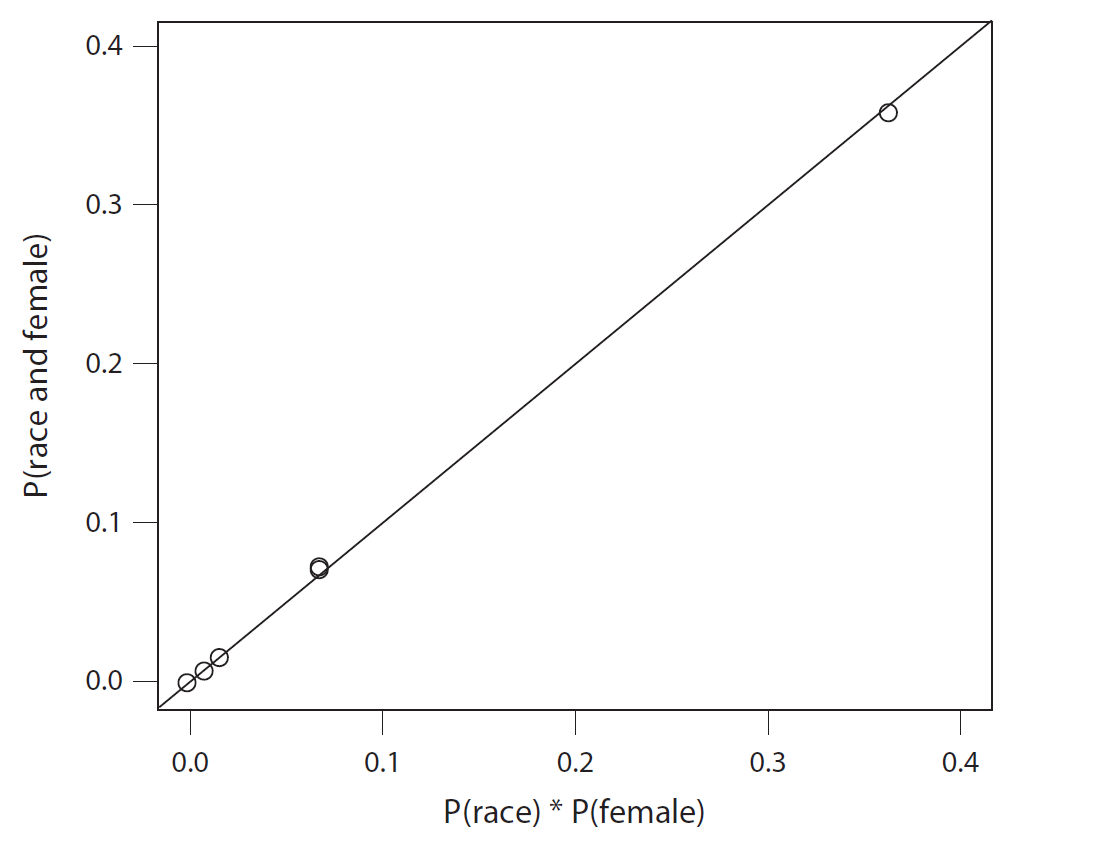
\includegraphics[scale=0.35]{../LaTex/img/ind_race_gender.png}
    \end{center}
    
    Recall that independence holds if the product of the probabilities equals the joint probability. In our case, we should have, taking as an example the black race, $P(\text{black and female}) = P(\text{black})P(\text{female})$.

    The scatter plot shows that the points fall neatly along the 45-degree line, implying that $P(\text{race})P(\text{female})$ (horizontal axis) and $P(\text{race and female})$ (vertical axis) are approximately equal. This means that race and gender are approximately independent in this sample of registered voters. That is,
    \begin{itemize}
        \item[] \centering \textit{The knowledge of a voter’s gender does not help us predict her race. \\
        Similarly, one’s race does not predict gender either.}
    \end{itemize}
    \end{solution}
    
    % \item \textbf{Joint Independence.}
    % \label{part:jointindependence}
    % Now, we examine joint independence among race, gender, and age group.
    % \begin{enumerate}
    %     \item Compute the product of marginal probabilities $P(\text{race}) \times P(\text{above 60}) \times P(\text{female})$.
    %     \item Compare this product to the three-way joint probabilities $P(\text{race and above 60 and female})$ using a scatter plot, by plotting the product probability on the $x$-axis and the three-way joint probability on the $y$-axis. Add a $45^\circ$ line to assess independence.
    % \end{enumerate}

    % \item \textbf{Conditional Independence.}
    % \label{part:conditionalindependence}
    % Next, we examine the conditional independence of race and gender, given age group.
    % \begin{enumerate}
    %     \item Compute the conditional joint probabilities $P(\text{race and above 60 | female})$.
    %     \item Compute the product of conditional marginal probabilities $P(\text{race | female}) \times P(\text{above 60 | female})$.
    %     \item Compare these values in a scatter plot, with $P(\text{race | female}) \times P(\text{above 60 | female})$ on the $x$-axis and $P(\text{race and above 60 | female})$ on the $y$-axis. Add a $45^\circ$ line to the plot and interpret the result.
    % \end{enumerate}

\end{enumerate}

\textbf{\textit{Hints}}

\begin{itemize}
    \item Use the R functions \texttt{prop.table()} and \texttt{table()}, and proper data subsetting if needed, to create the probability tables in parts \ref{part:marginal} to \ref{part:joint}.
    \item For scatter plots, use the \texttt{plot()} function with additional arguments like \texttt{xlab}, \texttt{ylab}, and \texttt{abline(0, 1)} for the $45^\circ$ line.
    \item You can validate your results by ensuring that the probabilities sum to 1 within their respective categories.
\end{itemize}



%%%
% Exercise 3
%%%



%%%
% Exercise 4
%%%



%%%
% Exercise 5
%%%


\end{document}




\end{document}
